% Autor: Leonhard Segger, Alexander Neuwirth
% Datum: 2017-10-30
\documentclass[
	% Papierformat
	a4paper,
	% Schriftgröße (beliebige Größen mit „fontsize=Xpt“)
	12pt,
	% Schreibt die Papiergröße korrekt ins Ausgabedokument
	pagesize,
	% Sprache für z.B. Babel
	ngerman
]{scrartcl}

% Achtung: Die Reihenfolge der Pakete kann (leider) wichtig sein!
% Insbesondere sollten (so wie hier) babel, fontenc und inputenc (in dieser
% Reihenfolge) als Erstes und hyperref und cleveref (Reihenfolge auch hier
% beachten) als Letztes geladen werden!

% Silbentrennung etc.; Sprache wird durch Option bei \documentclass festgelegt
\usepackage{babel}
% Verwendung der Zeichentabelle T1 (Sonderzeichen etc.)
\usepackage[T1]{fontenc}
% Legt die Zeichenkodierung der Eingabedatei fest, z.B. UTF-8
\usepackage[utf8]{inputenc}
% Schriftart
\usepackage{lmodern}
% Zusätzliche Sonderzeichen
\usepackage{textcomp}

% Mathepaket (intlimits: Grenzen über/unter Integralzeichen)
\usepackage[intlimits]{amsmath}
% Ermöglicht die Nutzung von \SI{Zahl}{Einheit} u.a.
\usepackage{siunitx}
% Zum flexiblen Einbinden von Grafiken (\includegraphics)
\usepackage{graphicx}
% Abbildungen im Fließtext
\usepackage{wrapfig}
% Abbildungen nebeneinander (subfigure, subtable)
\usepackage{subcaption}
% Funktionen für Anführungszeichen
\usepackage{csquotes}
% Zitieren, Bibliographie
\usepackage{biblatex}

% Verlinkt Textstellen im PDF-Dokument
\usepackage[unicode]{hyperref}
% "Schlaue" Referenzen (nach hyperref laden!)
\usepackage{cleveref}
% Zur Darstellung von Webadressen
\usepackage{url}
%chemische Formeln
\usepackage[version=4]{mhchem}
% siunitx: Deutsche Ausgabe, Messfehler getrennt mit ± ausgeben
\sisetup{
	locale=DE,
	separate-uncertainty
}
%\bibliography{6Mi_S2_25-10-2017_References}

\begin{document}
	
	\begin{titlepage}
		\centering
		{\scshape\LARGE Versuchsbericht zu \par}
		\vspace{1cm}
		{\scshape\huge E5 - Magnetische Suszeptibilität\par}
		\vspace{2.5cm}
		{\LARGE Gruppe 6Mi \par}
		\vspace{0.5cm}
		
		{\large Alexander Neuwirth (E-Mail: a\_neuw01@wwu.de) \par}
		{\large Leonhard Segger (E-Mail: l\_segg03@uni-muenster.de) \par}
		\vfill
		
		durchgeführt am 25.10.2017\par
		betreut von\par
		{\large Fabian Schöttke}
		
		\vfill
		
		{\large \today\par}
	\end{titlepage}
	\tableofcontents
	\newpage
	
	\section{Kurzfassung}
	Die Reaktion eines Stoffes auf ein Magnetfeld ist abhängig von der Volumensuszeptibilität $\xi_V$. Ist der Stoff diamagnetisch ($\xi_V<0$), so wird er vom Magneten schwach abgestoßen und ist er paramagnetisch ($\xi_V>0$), so wird sie schwach angezogen. Den Ferro- und Antiferromagnetismus haben wir in diesem Versuch nicht betrachtet.
	
	\section{Fermi Abschätzung zum Einfluss der Suszeptibilität auf die Oberfläche einer Flüssigkeit}
	\subsection{Methoden}
	Es ist zu erwarten, dass ein diamagnetischer Flüssigkeitsfilm über einem Magneten einen Berg ausbildet und ein paramagnetischer Flüssigkeitsfilm ein Tal ausbildet. 
	Um Rückschlüsse auf die Suszeptibilität von Flüssigkeiten zu untersuchen, wurde ein Laser auf eine Flüssigkeit in einer Petrischale gerichtet und die Reflexion des Lasers auf einer Wand beobachtet. Dann wurde unter der Petrischale ein Magnet hindurch bewegt. Aus der Änderung des Reflexionswinkels lässt sich dann die Höhe des Tal oder Berges über dem Magneten abschätzen. Untersucht wurde Wasser und mit Wasser verdünntes Manganchlorid.
	%TODO: Skizze mit Bezeichnungen aus dem Laborbuch
	\subsection{Ergebnisse}
	Bei Breite des Magneten $d \approx 1 \si{cm}$ , Ruhelage der Reflexion auf der Wand $b \approx 3 \si{m}$ und Abstand der Petrischale zur Wand $a \approx 6 \si{m}$ ergibt sich für die Auslenkung $\Delta y$ des Lasers auf der Wand: \newline
	$ \Delta y_\text{\ce{H2O}} \approx -7 \si{cm} \\
	\Delta y_\text{\ce{MnCl2}} \approx 15 \si{cm}$
	
	\begin{figure}[htb]
	  \centering
	    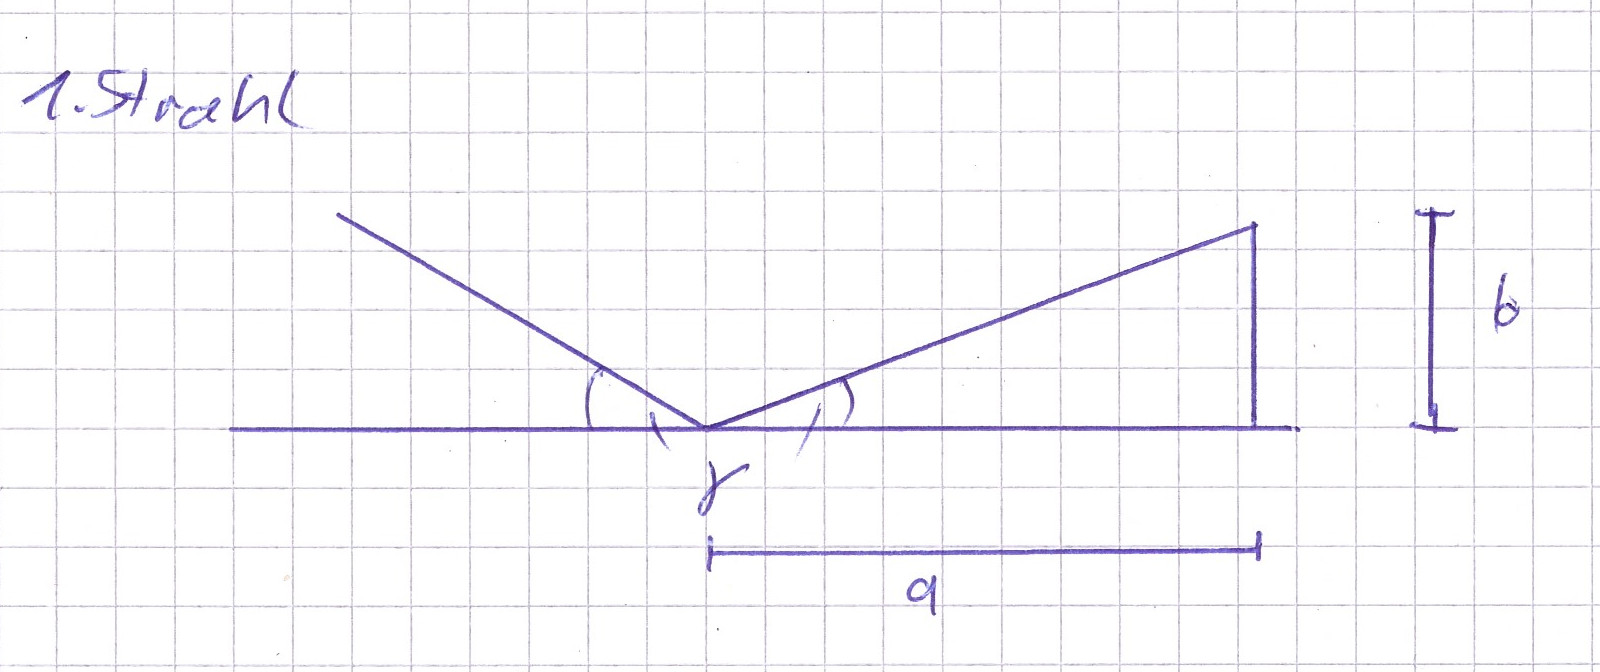
\includegraphics[width=0.6\textwidth]{Fermi1} 
	  \caption{Fermi Abschätzung Skizze Strahl 1}
	\end{figure}
		
	\begin{figure}[htb]
	  \centering
	    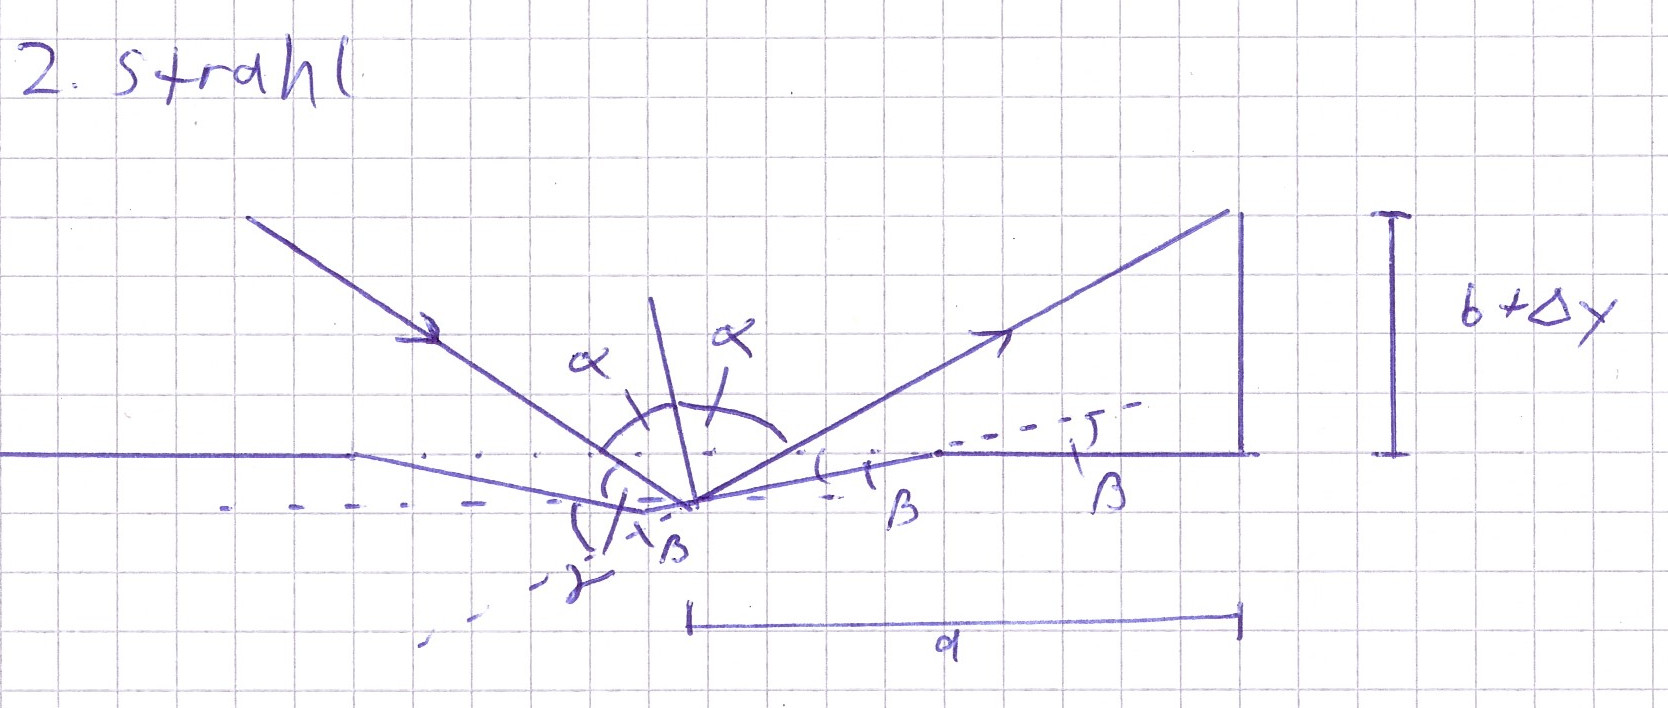
\includegraphics[width=0.6\textwidth]{Fermi2} 
	  \caption{Fermi Abschätzung Skizze Strahl 2}
	\end{figure}
	\begin{figure}[htb]
	  \centering
	    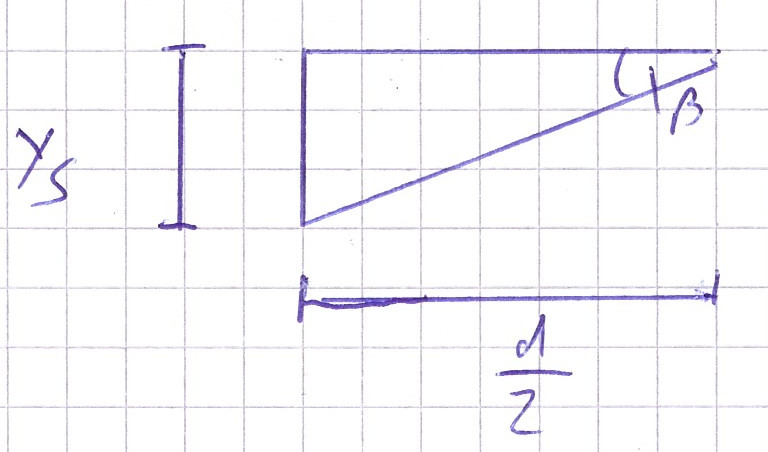
\includegraphics[width=0.6\textwidth]{Fermi3} 
	  \caption{Fermi Abschätzung Skizze Dreieck}
	\end{figure}

	\begin{gather*}
		\gamma = \arctan \left(\frac{b}{a}\right) \\
		\alpha = \ang{90} - \beta - \gamma \\
		\arctan \left(\frac{b+\Delta y}{a}\right) = \ang{180} - \gamma - 2\alpha \\
		\arctan \left(\frac{b+\Delta y}{a}\right) = \gamma + 2 \beta \\
		\arctan \left(\frac{b+\Delta y}{a}\right) =   \arctan \left(\frac{b}{a}\right) + 2 \beta \\
		\Rightarrow \beta = \frac{\arctan \left(\frac{b+\Delta y}{a}\right) -  \arctan \left(\frac{b}{a}\right)}{2} \\
		\Rightarrow y_\text{S} = \tan (\beta) \frac{d}{2}  \\
	\end{gather*}
	Setzt man die gemessenen Werte in die Formel ein so erhält man: $ y_{\text{S,\ce{H2O}}} = \SI{-0,0023}{ cm} $ und $y_{\text{S,\ce{MnCl2}}} = \SI{0,00495}{ cm} $. Das Wasser wird folglich abgestoßen und die Mangan-Chlorid-Lösung wird von dem Magneten angezogen.
	\subsubsection*{Unsicherheiten}
	Beim Aufstellen der Gleichung wurde die Approximatation verwendet, dass beide Reflektionen in gleichem Abstand zur Wand stattfinden. Dass dies kaum Einfluss auf das Ergebniss nimmt zeigt die folgende Rechnung:
	\begin{align*}
		\Delta x &= \tan (\gamma) y_\text{S} \\
		\Delta x &= \frac{b}{a} y_\text{S}
	\end{align*}
	Da unsere Schätzung von $a$, bzw. von dem Verhältnis $\frac{b}{a}$, eine größere Unsicherheit aufweißt, als der Fehler $\Delta x$, der bei der Näherung entsteht, ist dieser vernachlässigbar.



	\subsection{Schlussfolgerung}
	Zur Näherung der Verformung der Wasseroberfläche nutzen wir eine Fermi-Abschätzung. Dafür treffen wir die vereinfachende Annahme, dass der Berg bzw. das Tal eine Dreiecksform haben mit dem Ziel, die Höhe $h$ des Dreiecks zu bestimmen. Zugrunde legen wir das Reflexionsgesetz für die Reflexion des Lasers an der Tal-/Bergwand.
	
	\section{Bestimmung der Volumensuszeptibilität von Glas, Kohlenstoff und Graphit}
	\subsection{Methoden}
	\subsection{Ergebnisse und Diskussion}
	\subsection{Schlussfolgerung}
	
	\section{Untersuchung der gegenseitigen Reaktion von Magneten und Aluminium bei Relativbewegung}
	\subsection{Methoden}
	\paragraph{Magnetstab und Aluminiumplättchen}
	\paragraph{Aluminiumröhre und Permanentmagnet}
	\subsection{Ergebnisse}
	\subsection{Schlussfolgerung}
	%\printbibliography
\end{document}
